                                                                                                                                                                                                                                                                                                                                                                                                                                                                                                                                                                                                                                                                                                                                                                                                                                                                                                                                                                                                                                                                                                                                                                                                                                                                                                                                                                                                                                                                                                                                                                                                                                                                                                                                                                                                                                                                                                                                                                                                                                                                                                                                                                                                                                                                                                                                                                                                                                                                                                                                                                                                                                                                                                                                                                                                                                                                                                                                                                                                                                                                                                                                                                                                                                                                                                                                                                                                                                                                                                                                                                                                                                                                                                                                                                                                                                                                                                                                                                                                                                                                                                                                                                                                                                                                                                                                                                                                                                                                                                                                                                                                                                                                                                                                                                                                                                                                                                                                                                                                                                                                                                                                                                                                                                                                                                                                                                                                                                                                                                                                                                                                                                                                                                                                                                                                                                                                                                                                                                                                                                                                                                                                                                                                                                                                                                                                                                                                                                                                                                                                                                                                                                                                                                                                                                                                                                                                                                                                                                                             %2multibyte Version: 5.50.0.2890 CodePage: 65001
%\input{tcilatex}
%\input{tcilatex}
%\input{tcilatex}
%\input{tcilatex}


\documentclass[notes=show]{beamer}
%%%%%%%%%%%%%%%%%%%%%%%%%%%%%%%%%%%%%%%%%%%%%%%%%%%%%%%%%%%%%%%%%%%%%%%%%%%%%%%%%%%%%%%%%%%%%%%%%%%%%%%%%%%%%%%%%%%%%%%%%%%%%%%%%%%%%%%%%%%%%%%%%%%%%%%%%%%%%%%%%%%%%%%%%%%%%%%%%%%%%%%%%%%%%%%%%%%%%%%%%%%%%%%%%%%%%%%%%%%%%%%%%%%%%%%%%%%%%%%%%%%%%%%%%%%%
\usepackage{mathpazo}
\usepackage{hyperref}


\usepackage{graphicx}
%\usepackage[spanish]{babel}
\usepackage[latin1]{inputenc}
\usepackage{listings}
\usepackage{amsmath}
\usepackage{amsfonts}
\usepackage{amsxtra}
\usepackage{amstext}
\usepackage{amssymb}
\usepackage{latexsym}
\usepackage{subfigure}
\usepackage{eurosym}
\linespread{1.2}
\usepackage{multimedia}
\usepackage{dsfont} % for \mathds{N}
\usepackage{graphicx}
\usepackage{color,colortbl}
\usepackage{multirow}
\definecolor{clearBlue}{cmyk}{0.15,0.1,0,0.1}
\usepackage{bbm}

%TCIDATA{OutputFilter=LATEX.DLL}
%TCIDATA{Version=5.50.0.2890}
%TCIDATA{Codepage=65001}
%TCIDATA{<META NAME="SaveForMode" CONTENT="1">}
%TCIDATA{BibliographyScheme=Manual}
%TCIDATA{LastRevised=Sunday, April 01, 2012 14:26:41}
%TCIDATA{<META NAME="GraphicsSave" CONTENT="32">}

\newenvironment{stepenumerate}{\begin{enumerate}[<+->]}{\end{enumerate}}
\newenvironment{stepitemize}{\begin{itemize}[<+->]}{\end{itemize} }
\newenvironment{stepenumeratewithalert}{\begin{enumerate}[<+-| alert@+>]}{\end{enumerate}}
\newenvironment{stepitemizewithalert}{\begin{itemize}[<+-| alert@+>]}{\end{itemize} }
\usetheme{Singapore}

%\input{tcilatex}

\begin{document}

\title[Moment Inequalities]{Pakes Porter Ho Ishii (2011)\\ + \\Moment Inequalities in Binary Choice Problems (Based on Dickstein and Morales (2013))}
\author[MJ Dickstein]{Michael J. Dickstein \\
%EndAName
Stanford University}
\institute{Economics 258}
%\date[3/11/13]{March 11, 2013}
\maketitle


%--------------------------------------------------------------------------------
\begin{frame}
\frametitle{Moment Inequalities in Binary Choice Problems}

Based on Dickstein and Morales (2013)

\end{frame}

%--------------------------------------------------------------------------------
\begin{frame}
\frametitle{Sources of Error in Empirical Models}
\framesubtitle{A. Structural Error}

\begin{itemize}
	\item \textbf{Structural error}: component of the agent's payoff function known to the agent at the time of her decision but not observed by the econometrician.	
	\pause
	\begin{itemize}
	\item Typically assumed to be the single source of error in structural models.
	\item Economic theory does not generally place restrictions on its distribution. Therefore,
	\pause
	\begin{itemize}
		\item In order to avoid \textbf{endogeneity}, we assume independence between structural error and observed covariates
		\item In discrete choice models, the econometrician (arbitrarily) chooses its distribution (up to a finite parameter vector)
	\end{itemize}
\end{itemize}
\end{itemize}
\end{frame}
%--------------------------------------------------------------------------------
\begin{frame}
\frametitle{Sources of Error in Empirical Models}
\framesubtitle{Expectational Error}

\begin{itemize}
	\item \textbf{Expectational error}: Mismatch between (a) the expectations of payoffs agents use when making decisions and (b) future realized payoffs.
	\item Standard datasets usually contain information on \textit{ex post} realizations of payoff relevant variables but rarely incorporate information on expectations.
	\begin{itemize}
		\item Expectational error often contributes to the error term in empirical models.
	\end{itemize}
\end{itemize}
\end{frame}

%--------------------------------------------------------------------------------
\begin{frame}
\frametitle{Sources of Error in Empirical Models}
\framesubtitle{Expectational Error}

\begin{itemize}
	\item Economic theory places restrictions on the distribution of expectational error. 
	\item The rational expectations assumption implies that:
	\begin{itemize}
	 	\item Expectational error is mean independent of the unobserved expectation (analogous to the classical \textbf{error-in-variables}).
		\item Expectational error is correlated with observed covariate (\textbf{endogeneity})
		\item Any variable in the agent's information set is a valid \textbf{instrumental variable}.
	\end{itemize}	
\end{itemize}
\end{frame}

%--------------------------------------------------------------------------------
\begin{frame}
\frametitle{Example: Export Decision}
\framesubtitle{Agents' Information and Expectations}

Daniel owns a small winery in Chile and is wondering whether he should try to export to Venezuela. To access customers in this market, Daniel needs to participate in a wine trade fair to be organized in June 2001 in Caracas. Daniel needs to make a decision by December 31, 2000.\\
\bigskip
Daniel has information on shipping costs and does not face any other export costs.\\
\bigskip
Daniel does not know the exact sales revenues he will obtain if he attends the fair.  
\end{frame}

%--------------------------------------------------------------------------------
\begin{frame}
\frametitle{Example: Export Decision}
\framesubtitle{Agents' Information and Expectations}

Using the information available to him (sales revenue of competitors, demand predictions, current political unrest, nominal exchange rate, etc) Daniel must form an \textbf{expectation} about his potential export revenues.\\
\bigskip
Daniel's choice over whether to attend the fair (or not) is a \textbf{binary} choice. He will attend the fair if his \textbf{expected} sales revenues net of shipping costs are positive.
\end{frame}

%--------------------------------------------------------------------------------
\begin{frame}
\frametitle{Example: Export Decision}
\framesubtitle{Econometrician's Information}
\begin{itemize}
\item The Chilean Customs Agency provides a dataset on the annual country-specific \textbf{realized} sales revenues obtained by each Chilean wine producer during 1995-2005
\item The econometrician assumes that shipping costs are a linear function of the distance between Santiago de Chile and Caracas (distance known).
\item The econometrician does not know: (a) the exact shipping cost per mile that Daniel will face if he chooses to export; (b) the expectation that Daniel had on December 31, 2000 about the revenue he would obtain in 2001 if he were to attend the fair.
\end{itemize}
\end{frame}
%--------------------------------------------------------------------------------
\begin{frame}
\frametitle{Example: Export Decision}
\framesubtitle{How shall the econometrician handle the unobserved shipping costs?}

The shipping costs form the \textbf{structural error}; i.e. variables known to Daniel at the time of his decision, but unobserved by the econometrician.\\
\bigskip
The econometrician assumes that these shipping costs are normally distributed around a mean that he will estimate, and sets the variance to an arbitrary constant.
\end{frame}
%-----------------------------------------------------------------------------------
\begin{frame}
\frametitle{Example: Export Decision}
\framesubtitle{How should the econometrician handle the unobserved expectations?}

Options:
\begin{itemize}
	\item 1. Compute Daniel's unobserved expectations. Assumptions:
	\begin{itemize}
		\item Realized revenues are observed without error.
		\item All information Daniel used to form his expectation is available to the econometrician (i.e. Daniel's information set is observable); 
		\item Daniel has rational expectations.
	\end{itemize}
	\pause
	\item 2. Assume that Daniel's expectations are identical to the observed measurement of realized revenues. Assumptions:
	\begin{itemize}	
		\item Realized revenues are observed without error.
		\item Daniel has perfect foresight.
	\end{itemize}
\end{itemize}
\end{frame}
%-----------------------------------------------------------------------------------
\begin{frame}
\frametitle{Example: Export Decision}
\framesubtitle{How should the econometrician handle the unobserved expectations?}

Options:
\begin{itemize}
	\item 3. Use the ex post measurement of potential revenue as a proxy for the unobserved expectation. Assumptions:
	\begin{itemize}
		\item Daniel has rational expectations.
	\end{itemize}
\end{itemize}
Option 3 imposes fewer assumption but introduces \textbf{errors-in-variables}.
\end{frame}
%--------------------------------------------------------------------------------
\begin{frame}
\frametitle{Goal of the paper}

Illustrate how to use \textbf{moment inequalities} to \textbf{identify and estimate the index coefficients}
of \textbf{binary choice models} allowing for \textbf{structural errors}
and \textbf{errors-in-variables.}

\end{frame}
%--------------------------------------------------------------------------------
\section{Errors}
%--------------------------------------------------------------------------------
\begin{frame}
\frametitle{Expectational and Measurement Error}

\begin{itemize}
	\item The payoff function of agent $i$ for alternative $j$ is
	\begin{align*}
	U_{j} = \beta\mathcal{E}[X_{j}|\mathcal{J}]+\nu_{j}= \beta X^{*}_{j}+\nu_{j},\qquad j \in \{0,1\}.
	\end{align*}
	\item We denote the expectational error as
	\begin{align*}
	\varepsilon_{j} = \beta X_{j}-\beta \mathcal{E}[X_{j}|\mathcal{J}],
	\end{align*}
	and rewrite payoff function as
	\begin{align*}
	U_{j} = \beta X_{j}+\nu_{j}-\varepsilon_{j}.
	\end{align*}
	\item If $\mathcal{E}[\cdot]$ = $\mathbbm{E}[\cdot]$, then
	\begin{equation*}
	\mathbbm{E}[\varepsilon_{j}|X^{*}_{j}]=0,\qquad\text{ and }\qquad\mathbbm{E}[\varepsilon_{j}|X_{j}]\neq0.
	\end{equation*}
\end{itemize}
\end{frame}

\begin{frame}
\frametitle{Expectational and Measurement Error}

\begin{itemize}
	\item If $\mathcal{E}[\cdot]$ = $\mathbbm{E}[\cdot]$, then
	\begin{equation*}
	\mathbbm{E}[\varepsilon_{j}|X^{*}_{j}]=0,\qquad\text{ and }\qquad\mathbbm{E}[\varepsilon_{j}|X_{j}]\neq0.
	\end{equation*}
	\item Rational expectations assumption $\Longrightarrow$ Errors-in-variables assumption.
	\item For any $Z\in\mathcal{J}$, $\mathbbm{E}[\varepsilon_{j}|Z]=0$ $\Longrightarrow$ Z is an IV.
\end{itemize}
\end{frame}

%--------------------------------------------------------------------------------
\section{Statistical Model}
%--------------------------------------------------------------------------------
\begin{frame}
\frametitle{Binary Choice Model}
\framesubtitle{Agents' decisions}

\begin{itemize}
	\item Utility of individual $i$ for any alternative $j$ $\in$ $\{0,1\}$ is
	\begin{align*}
	U_{j}=\beta X^{*}_{j} + \nu_{j}.
	\end{align*}
	\item For any $j$, each dummy variable $d_{j}$ is defined as
	\begin{align*}
	d_{j} = \mathbbm{1}\{\Delta U_{j}\geq 0\},\qquad\Delta U_{j} = U_{j}-U_{j'}
	\end{align*}
	\item Therefore, for any $j$ $\in$ $\{0,1\}$, we can write the individual revealed preference inequality as
	\begin{align*}
	d_{j} \cdot (\beta\Delta X^{*}_{j}+\Delta\nu_{j})\geq 0.
	\end{align*}
	\item The term $\beta\Delta X^{*}_{j}$ is the index function and $\beta$ is the parameter we want to identify and estimate. We assume this index function is \textbf{linear in covariates}.
\end{itemize}
\end{frame}
%--------------------------------------------------------------------------------
\begin{frame}
\frametitle{Binary Choice Model}
\framesubtitle{Measurement model}

\begin{itemize}
	\item Without loss of generality, we can write 
	\begin{align*}
	\beta\Delta X^{*}_{j} = \beta_{1}\Delta X^{*}_{1j} + \beta_{2}\Delta X^{*}_{2j},
	\end{align*}
	where $\beta_{1}\Delta X^{*}_{1j}$ is measured without error,
	\begin{align*}
	\beta_{1}\Delta Z_{1j} = \beta_{1}\Delta X^{*}_{1j},
	\end{align*}
	and $\beta_{2}\Delta X^{*}_{2j}$ is measured with error,
	\begin{align*}
	\beta_{2}\Delta X_{j} = \beta_{2}\Delta X^{*}_{2j}+\Delta\varepsilon_{j}.
	\end{align*}
\end{itemize}
\end{frame}

%--------------------------------------------------------------------------------
\begin{frame}
\frametitle{Binary Choice Model}
\framesubtitle{Measurement model}

\begin{itemize}
	\item Therefore, we can write the individual revealed preference inequality as
	\begin{align*}
	d_{j} \cdot (\beta_{1}\Delta Z_{1j}+\beta_{2}\Delta X_{j}+\Delta\nu_{j}+\Delta\varepsilon_{j})\geq 0.
	\end{align*}
	\item In addition, we observe a vector $\Delta Z_{2j}$ and denote $\Delta Z_{j}$ = $(\Delta Z_{1j},$ $\Delta Z_{2j})$.
\end{itemize}
\end{frame}
%--------------------------------------------------------------------------------
\begin{frame}
\frametitle{Binary Choice Model}
\framesubtitle{Assumptions}

\textbf{Assumption 1} \textit{The random variable $\Delta\nu_{j}$ is independent of the random vector $(\Delta Z_{j},\Delta X^{*}_{j})$: 
\begin{align*}
F_{\nu}(\Delta\nu_{j}|(\Delta Z_{j},\Delta X^{*}_{j}))=F_{\nu}(\Delta\nu_{j}).
\end{align*}}
\textbf{Assumption 2} \textit{The marginal distribution function of $\Delta\nu_{j}$ is known up to a scale parameter, log concave, has mean zero, and, for any $y$ in the support of $\Delta\nu_{j}$, verifies the following property:
\begin{align*}
\frac{\partial^{2}\mathbbm{E}[\Delta\nu_{j}|\Delta\nu_{j}\geq y]}{\partial y^{2}}\geq 0.
\end{align*}}
\textbf{Assumption 3} \textit{The distribution of $\Delta\varepsilon_{j}$ conditional on $(\Delta X^{*}_{j},\Delta Z_{j},\Delta \nu_{j})$ has support $(-\infty,$ $\infty)$ and mean zero:
\begin{align*}
\mathbbm{E}[\Delta\varepsilon_{j}|\Delta X^{*}_{j},\Delta Z_{j},\Delta\nu_{j}]=0.
\end{align*}}
\end{frame}
%--------------------------------------------------------------------------------
\begin{frame}
\frametitle{Binary Choice Model}
\framesubtitle{Comments on Assumptions}

\begin{itemize}
	\item Assumption 1 imposes that the endogeneity problem is exclusively due to measurement error.
	\begin{itemize}
		\item It excludes models with random coefficients.
	\end{itemize}
	\item Both the normal and the logistic distribution verify Assumptions 1 and 2. 
	\begin{itemize}
		\item Our model generalizes the probit and logit model to allow for classical measurement error in covariates.
	\end{itemize}
\end{itemize}
\end{frame}

%--------------------------------------------------------------------------------
\begin{frame}
\frametitle{Binary Choice Model}
\framesubtitle{Comments on Assumptions}

\begin{itemize}
	\item Assumption 3 imposes the classical error-in-variables assumption.
	\begin{itemize}
		\item It does not impose a parametric assumption on the marginal distribution of the measurement error.
		\item It does not require full independence between the measurement error and the vector $(\Delta X^{*}_{j},$ $\Delta Z_{j},$ $\Delta\nu_{j})$
	\end{itemize}
	\item If $\Delta\varepsilon_{j}$ captures expectational error and we assume rational expectations, the only additional restriction that Assumption 3 imposes is that $\Delta Z_{2j}$ $\in$ $\mathcal{J}$.
\end{itemize}
\end{frame}

%--------------------------------------------------------------------------------
\begin{frame}
\frametitle{Binary Choice Model}
\framesubtitle{Identification}

\begin{itemize}
	\item Data are informative about the conditional density of $(d_{j},\Delta X_{j})$ given $\Delta Z_{j}$. 
	\begin{align*}
	\mathcal{P}(d_{j},\Delta X_{j}|\Delta Z_{j})&=\int_{X^{*}}f(d_{j},\Delta X_{j}|\Delta Z_{j},\Delta X^{*}_{j};\beta)f(\Delta X^{*}_{j}|\Delta Z_{j})d\Delta X^{*}_{j},\\
	&=\int_{X^{*}}f(d_{j}|\Delta X^{*}_{j};\beta)f(\Delta X_{j}|\Delta Z_{j},\Delta X^{*}_{j})f(\Delta X^{*}_{j}|\Delta Z_{j})d\Delta X^{*}_{j},
	\end{align*}
\end{itemize}
\end{frame}

%--------------------------------------------------------------------------------
\begin{frame}
\frametitle{Binary Choice Model}
\framesubtitle{Identification}

\begin{itemize}
	\item With
	\begin{align*}
	f(d_{j}|\Delta X^{*}_{j};\beta)=\int_{\Delta\nu}\mathbbm{1}\{\Delta\nu_{j}\geq-\beta\Delta X^{*}_{j}\}f(\Delta\nu_{j})d\Delta\nu_{j},
	\end{align*}
	and
	\begin{align*}
	f(\Delta X^{*}_{j}|\Delta Z_{j})=\frac{f(\Delta Z_{j}|\Delta X^{*}_{j})f(\Delta X^{*}_{j})}{\int_{\Delta X^{*}}f(\Delta Z_{j}|\Delta X^{*}_{j})f(\Delta X^{*}_{j})d\Delta X^{*}_{j}}.
	\end{align*}
	\item Assumptions 1 to 3 impose no restriction on $f(\Delta Z_{j}|\Delta X^{*}_{j})$ and $f(\Delta X^{*}_{j})$.
	\item Assumption 3 restricts the mean of $f(\Delta X_{j}|\Delta Z_{j},\Delta X^{*}_{j})$.
\end{itemize}
\end{frame}

%--------------------------------------------------------------------------------
\begin{frame}
\frametitle{Binary Choice Model}
\framesubtitle{Identification}

\begin{itemize}
	\item The parameter vector $\beta$ is set-identified, not point-identified.
	\item Intuition:
	\begin{itemize}
		\item Given a distribution $f(\Delta\nu_{j})$, the parameter vector $\beta$ captures choice sensitivity to differences in the covariates $\Delta X^{*}_{j}$.
		\item If $\Delta X^{*}_{j}$ was observed, this sensitivity could be measured directly and $\beta$ would be point identified.
		\item However, $\Delta X^{*}_{2j}$ is unobserved: the econometrician only observes the vector $\Delta X_{j}$, which is known to have the same mean as $\Delta X^{*}_{j}$.
	\end{itemize}
\end{itemize}
\end{frame}

%--------------------------------------------------------------------------------
\begin{frame}
\frametitle{Binary Choice Model}
\framesubtitle{Identification}

\begin{itemize}
	\item Intuition: (continued)
	\begin{itemize}
		\item This mean restriction is not enough for point identification. Example: If choices are more sensitive to variation in $\Delta X^{(1)}_{j}$ than in $\Delta X^{(2)}_{j}$, it could be because: (a) the $\beta$ coefficient on $\Delta X^{(1)}_{j}$ is higher than that on $\Delta X^{(2)}_{j}$; or (b) the variance of $\Delta X^{(1)}_{j}$ conditional on $\Delta X^{*(1)}_{j}$ is lower than the variance of $\Delta X^{(2)}_{j}$ conditional on $\Delta X^{*(2)}_{j}$.
		\item Even if $\Delta Z_{2j}$ is fully independent of $\Delta\varepsilon_{j}$, the parameter $\beta$ is still set identified (Chesher (2010))
	\end{itemize}
\end{itemize}
\end{frame}

%--------------------------------------------------------------------------------	
\section{Simulation}
%--------------------------------------------------------------------------------
\begin{frame}
\frametitle{Simulation Exercise}

\begin{itemize}
	\item The utility function is:
	\begin{align*}
	U_{j}=\beta^{(1)}X^{*(1)}_{j} + \beta^{(2)}X^{*(2)}_{j} + \beta^{(3)}X^{*(3)}_{j}+ \nu_{j},\quad j=\{0,1\},
	\end{align*}
	with $\beta$ = $\mathbf{(0.5,0.5,0.25)}$ and
	\begin{align*}
	\nu_{j}\backsim\mathbbm{N}(0,\sigma_{\nu}^{2}),\qquad\sigma_{\nu}=1.
	\end{align*}
	\pause
	\item Both $X^{*(1)}_{j}$ and $X^{*(3)}_{j}$ are measured without error: $Z_{1j}$ = $(X^{*(1)}_{j},X^{*(3)}_{j})$.
	\item $X^{*(2)}_{j}$ is measured with error:
	\begin{align*}
	X_{j}=X^{*(2)}_{j}+\epsilon^{x}_{j},\qquad\epsilon^{x}_{j}\backsim\mathbbm{N}(0,\sigma_{\epsilon^{x}}^{2}),\qquad\sigma_{\epsilon^{x}}^{2}=0.2.
	\end{align*}
	 \item We generate $Z_{2j}$ as a second measurement of $X^{*(2)}_{j}$:
	 \begin{align*}
	Z_{2j}=X^{*(2)}_{j}+\epsilon^{z}_{j},\qquad\epsilon^{z}_{j}\backsim\mathbbm{N}(0,\sigma_{\epsilon^{z}}^{2}),\qquad\sigma_{\epsilon^{z}}^{2}=0.02.
	\end{align*}
\end{itemize}
\end{frame}
%--------------------------------------------------------------------------------
\section{Moment Inequalities}
%--------------------------------------------------------------------------------
\begin{frame}
\frametitle{Conditional Moment Inequalities}

\begin{itemize}
	\item We first derive two types of moment inequalities conditional on the instrumental variable $\Delta Z_{j}$.
	\item \textit{Score Function Moment Inequalities}
	\begin{align*}
	\mathcal{M}_{s}(Z,j;\beta)=\mathbbm{E}\Bigg[d_{j}\frac{F_{\nu}\big(-(\beta_{1}\Delta Z_{1j}+\beta_{2}\Delta X_{j})\big)}{1-F_{\nu}\big(-(\beta_{1}\Delta Z_{1j}+\beta_{2}\Delta X_{j})\big)}-d_{j'}\Big|Z\Bigg]\geq 0.
	\end{align*}
	\item \textit{Revealed Preference Moment Inequalities}
          \begin{align*}
	&\hspace{1.6in}\mathcal{M}_{r}(Z,j;\beta)=\mathbbm{E}\Big[d_{j}(\beta_{1}\Delta Z_{1j}+\beta_{2}\Delta X_{j})+\nonumber\\
	&d_{j'}\mathbbm{E}\big[\Delta\nu_{j'}|\Delta\nu_{j'}\geq-(\beta_{1}\Delta Z_{1j'}+\beta_{2}\Delta X_{j'})\big]\Big|Z\Big]\geq 0.
	\end{align*}
	\item For any $Z$ and $j$, $\mathcal{M}_{s}(Z,j;\beta^{*})$ $\geq$ $0$ and $\mathcal{M}_{r}(Z,j;\beta^{*})$ $\geq$ $0$.

\end{itemize}
\end{frame}
%--------------------------------------------------------------------------------
\begin{frame}
\frametitle{Unconditional Moment Inequalities}

\begin{itemize}
	\item The derive the same two types of unconditional inequalities.
	\item \textit{Score Function Moment Inequalities}
	\small
	\begin{align*}
	\mathcal{M}^{q}_{s}(\beta)=\mathbbm{E}\Bigg[\sum_{j\in\{0,1\}}\Bigg\{\Psi_{q}(\Delta Z_{j})\Bigg(d_{j}\frac{F_{\nu}\big(-(\beta_{1}\Delta Z_{1j}+\beta_{2}\Delta X_{j})\big)}{1-F_{\nu}\big(-(\beta_{1}\Delta Z_{1j}+\beta_{2}\Delta X_{j})\big)}-d_{j'}\Bigg)\Bigg\}\Bigg]\geq 0,
	\end{align*}
	\normalsize
	\item \textit{Revealed Preference Moment Inequalities}
	\small
	\begin{align*}
	\mathcal{M}^{q}_{r}(\beta)=\mathbbm{E}\Bigg[\sum_{j\in\{0,1\}}\Bigg\{\Psi_{q}(\Delta &Z_{j})\Bigg(d_{j}(\beta_{1}\Delta Z_{1j}+\beta_{2}\Delta X_{j})\nonumber\\
	&+d_{j'}\mathbbm{E}\big[\Delta\nu_{j'}|\Delta\nu_{j'}\geq-(\beta_{1}\Delta Z_{1j'}+\beta_{2}\Delta X_{j'})\big]\Bigg)\Bigg\}\Bigg]\geq 0.
	\end{align*}
	\normalsize
	\item The set of functions $\{\Psi_{q}(\Delta Z_{j}),$ $q$ $\in$ $Q\}$ groups different values of $\Delta Z_{j}$ into different unconditional moment inequalities. We call them \textit{instrument functions}.
\end{itemize}
\end{frame}

%--------------------------------------------------------------------------------
\begin{frame}
\frametitle{Instrument Functions}

\begin{itemize}
	\item As an example, in the particular case in which $\Delta Z_{j}$ is a $2\times 1$ vector, the matrix $Q$ defines 4 instrument functions:
	\begin{align*}
	\Psi_{1}(\Delta Z_{j})&=\mathbbm{1}\{\Delta Z_{1j}\geq0\}\mathbbm{1}\{\Delta Z_{2j}\geq0\},\\
	\Psi_{2}(\Delta Z_{j})&=\mathbbm{1}\{\Delta Z_{1j}\geq0\}\mathbbm{1}\{\Delta Z_{2j}<0\},\\
	\Psi_{3}(\Delta Z_{j})&=\mathbbm{1}\{\Delta Z_{1j}<0\}\mathbbm{1}\{\Delta Z_{2j}\geq0\},\\
	\Psi_{4}(\Delta Z_{j})&=\mathbbm{1}\{\Delta Z_{1j}<0\}\mathbbm{1}\{\Delta Z_{2j}<0\}.
	\end{align*}
\end{itemize}
\end{frame}
%--------------------------------------------------------------------------------
\begin{frame}
\frametitle{Identified Sets}

\begin{itemize}
	\item The identified sets defined by these sets of inequalities are
	\begin{align*}
	\Omega(\mathcal{M}_{s})&=\{\beta\in\Gamma_{\beta}: \mathcal{M}^{q}_{s}(\beta)\geq 0, q\in Q\},\\
	\Omega(\mathcal{M}_{r})&=\{\beta\in\Gamma_{\beta}: \mathcal{M}^{q}_{r}(\beta)\geq 0, q\in Q\},\\
	\Omega(\mathcal{M})&=\{\beta\in\Gamma_{\beta}: (\mathcal{M}^{q}_{s}(\beta); \mathcal{M}^{q}_{r}(\beta))\geq 0,  q\in Q\}.
	\end{align*}
\end{itemize}
\end{frame}
%--------------------------------------------------------------------------------
\begin{frame}
\frametitle{Properties of the Identified Sets}

All the following properties condition on Assumptions 1, 2, and 3.
\begin{enumerate}
	\item $\Omega(\mathcal{M})$ $\subseteq$ $\Omega(\mathcal{M}_{s})$ and $\Omega(\mathcal{M})$ $\subseteq$ $\Omega(\mathcal{M}_{r})$;
	\item $\beta^{*}$ $\in$ $\Omega(\mathcal{M})$;
	\item If $\bar{\bar{\sigma}}^{2}_{\varepsilon}$ $\geq$ $\bar{\sigma}^{2}_{\varepsilon}$, then, $\Omega(\mathcal{M}_{s}|\bar{\sigma}^{2}_{\varepsilon})$ $\subseteq$ $\Omega(\mathcal{M}_{s}|\bar{\bar{\sigma}}^{2}_{\varepsilon})$, $\Omega(\mathcal{M}_{r}|\bar{\sigma}^{2}_{\varepsilon})$ $\subseteq$ $\Omega(\mathcal{M}_{r}|\bar{\bar{\sigma}}^{2}_{\varepsilon})$, and $\Omega(\mathcal{M}|\bar{\sigma}^{2}_{\varepsilon})$ $\subseteq$ $\Omega(\mathcal{M}|\bar{\bar{\sigma}}^{2}_{\varepsilon})$
	\item $\Omega(\mathcal{M}_{s}),$ $\Omega(\mathcal{M}_{r}),$ and $\Omega(\mathcal{M})$ are convex.
	\item If $\Delta X_{j}$ = $\Delta X^{*}_{2j}$; and, for every $q$ $\in$ $Q$ and
	\begin{align*}
	\mathbbm{E}\Bigg[\sum_{j\in\{0,1\}}\Psi_{q}(\Delta Z_{j})\Bigg] \neq 0,
	\end{align*}
	then $\Omega(\mathcal{M}_{s})$ = $\Omega(\mathcal{M})$ = $\beta^{*}$.
	\item If $var(X-Z)$ $\approx$ $0$, then $\Omega(\mathcal{M}_{s})$, $\Omega(\mathcal{M}_{r})$, and $\Omega(\mathcal{M})$ are all closed and bounded.
\end{enumerate}
\end{frame}
%--------------------------------------------------------------------------------
\begin{frame}
\frametitle{Simulation Exercise: Moment Inequalities Estimator}

\begin{figure}[h!]
\centering 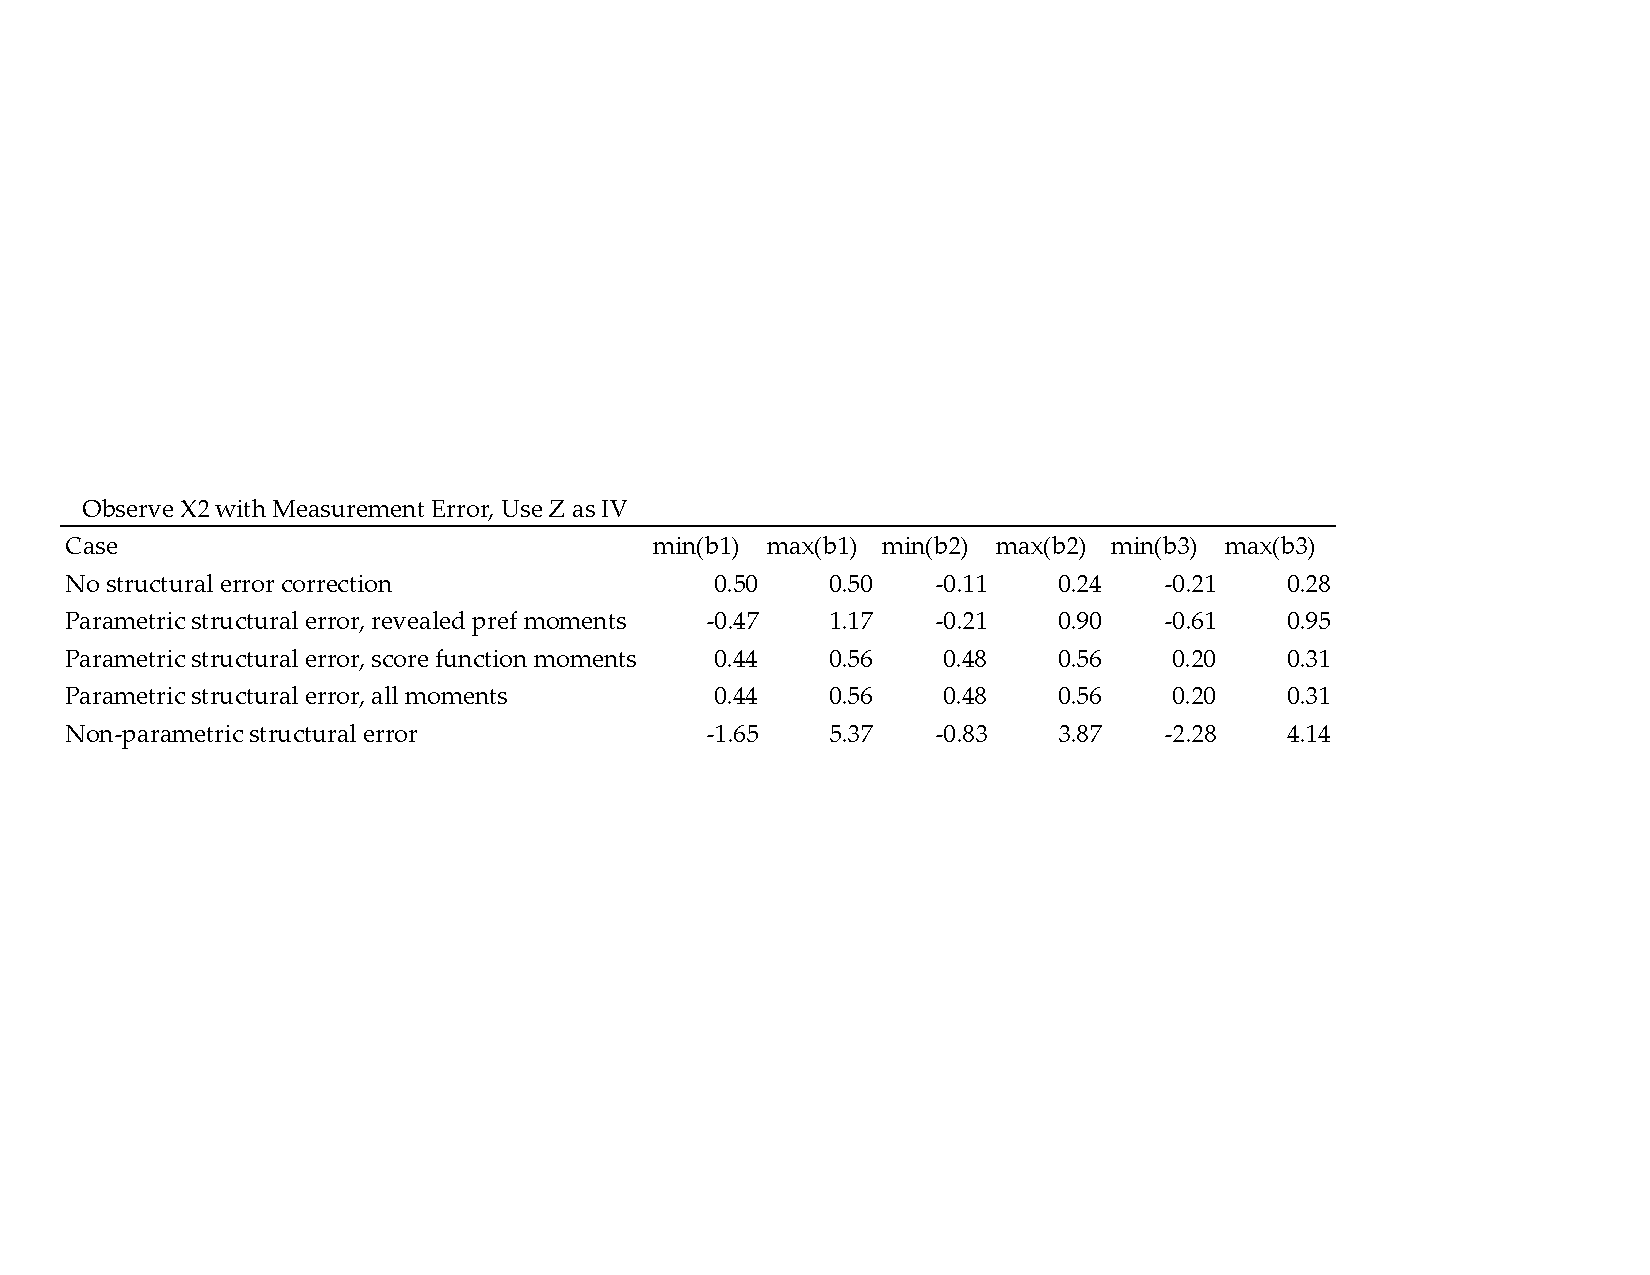
\includegraphics[width=1\linewidth]{id_sets_table.pdf}
\end{figure}

\end{frame}
%--------------------------------------------------------------------------------
\begin{frame}
\frametitle{Simulation Exercise: Moment Inequalities Estimator}

\begin{figure}[h!]
\centering 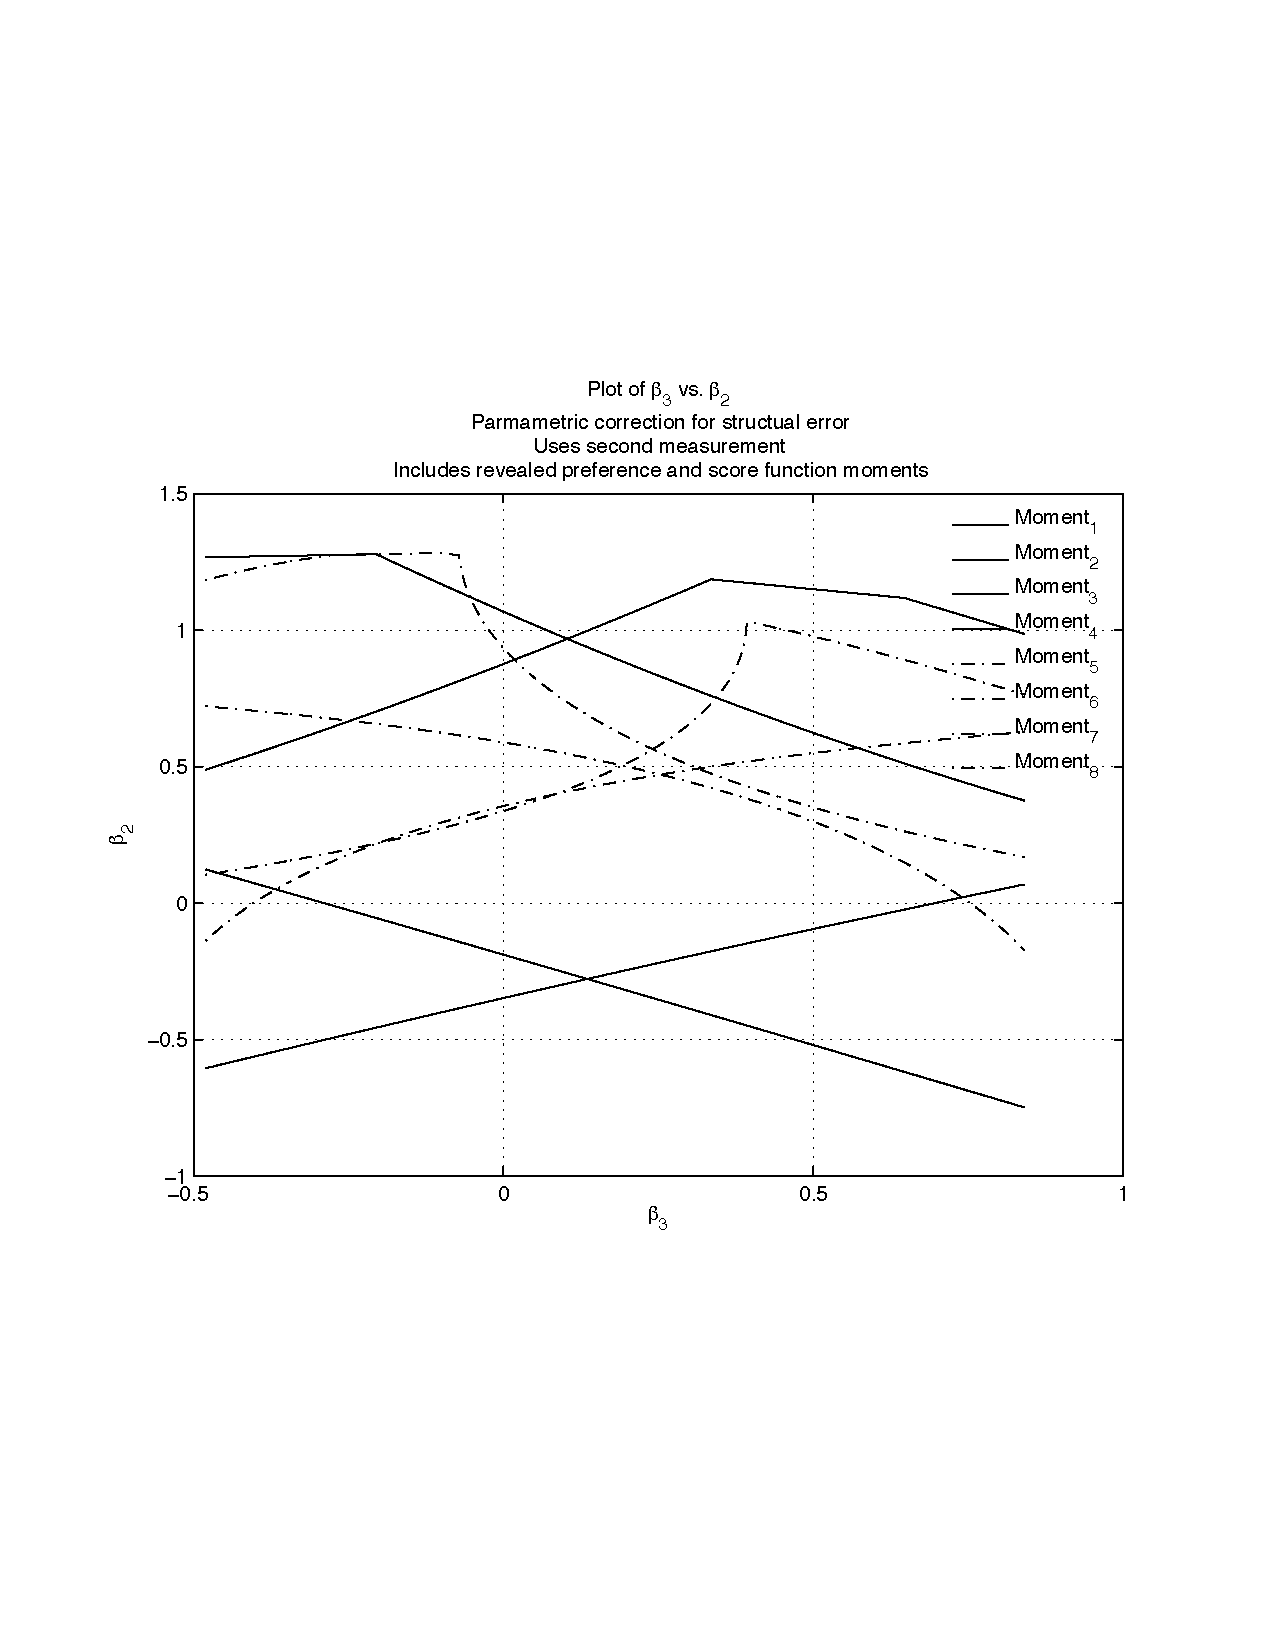
\includegraphics[width=.85\linewidth]{id_set_plots_all.pdf}
\end{figure}

\end{frame}
%--------------------------------------------------------------------------------
\begin{frame}
\frametitle{Simulation Exercise: Moment Inequalities Estimator}

\begin{figure}[h!]
\centering \includegraphics[width=.85\linewidth]{id_set_region_rp.pdf}
\end{figure}

\end{frame}

%--------------------------------------------------------------------------------
\begin{frame}
\frametitle{Simulation Exercise: Moment Inequalities Estimator}

\begin{figure}[h!]
\centering 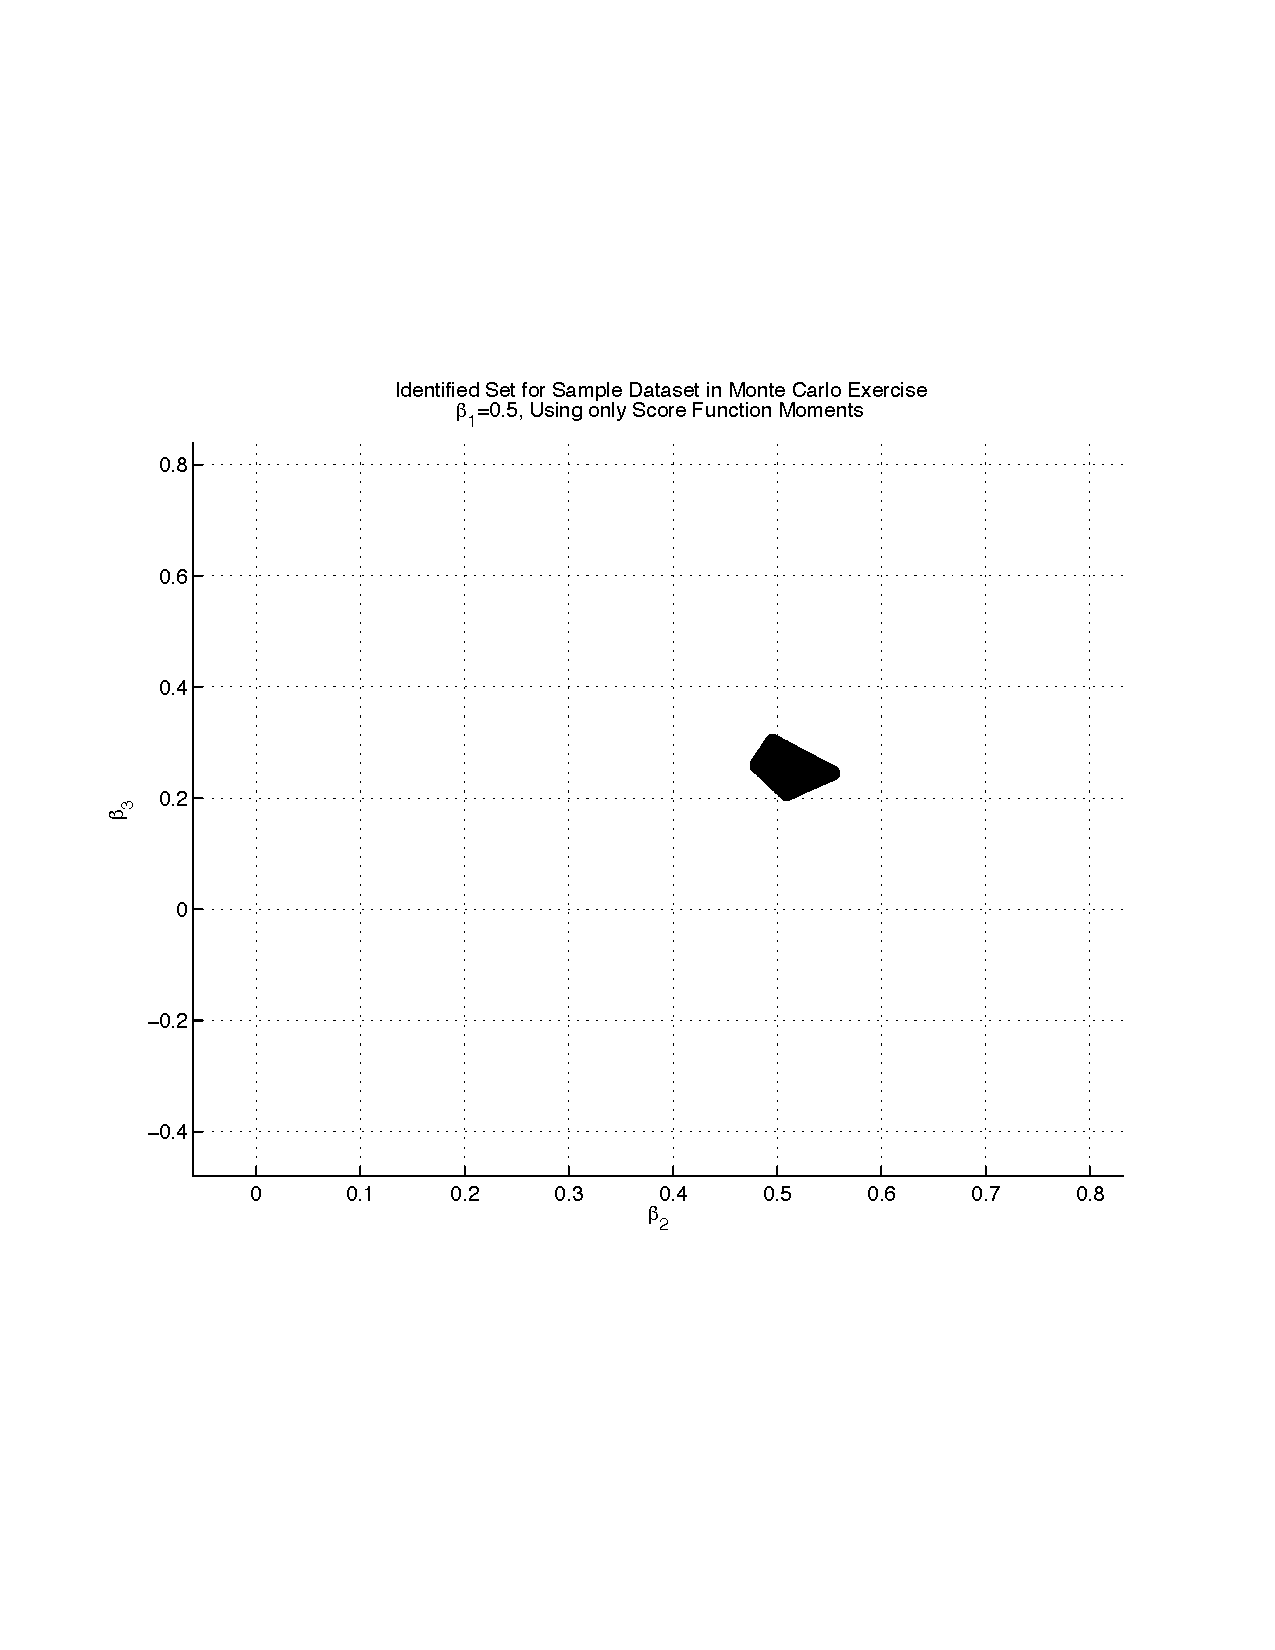
\includegraphics[width=.85\linewidth]{id_set_region_sf.pdf}
\end{figure}

\end{frame}
%--------------------------------------------------------------------------------
\begin{frame}
\frametitle{Simulation Exercise: Moment Inequalities Estimator}

\begin{figure}[h!]
\centering 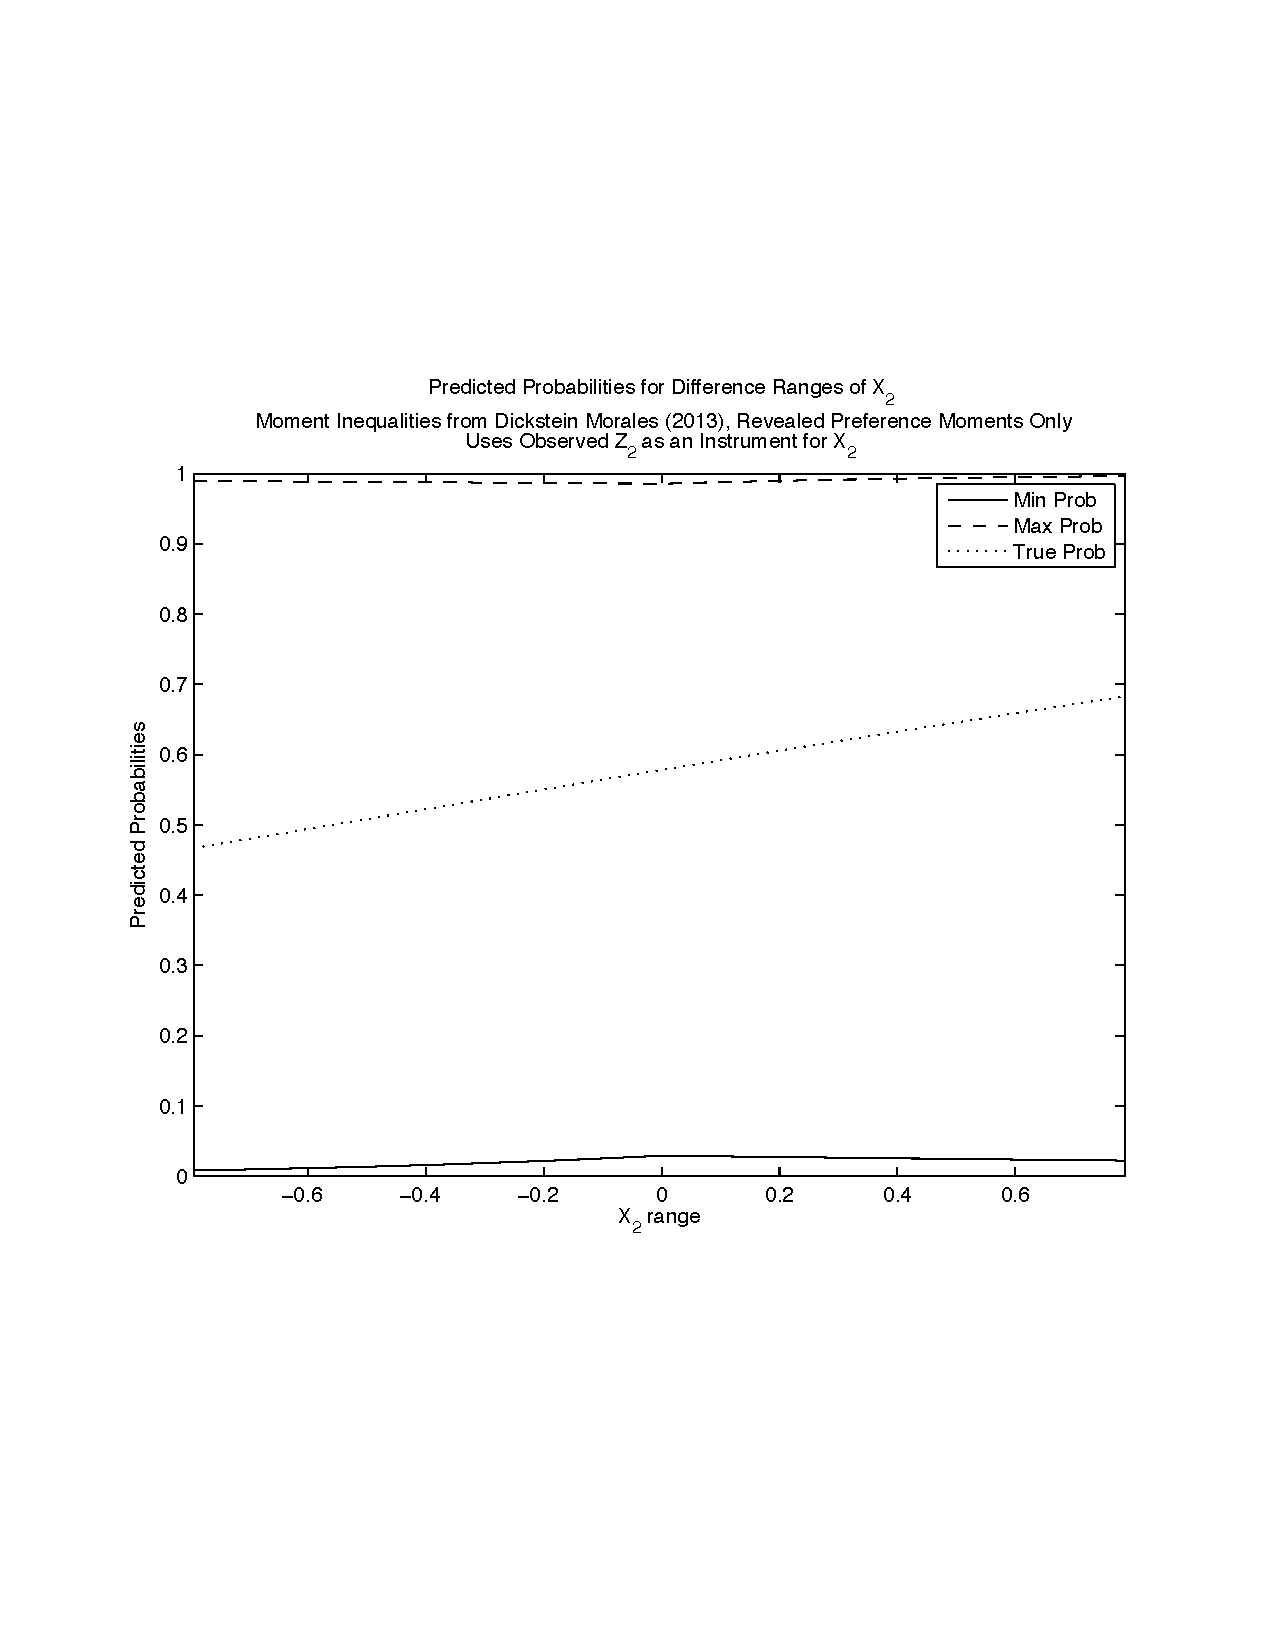
\includegraphics[width=.85\linewidth]{pred_prob_rp.pdf}
\end{figure}

\end{frame}

%--------------------------------------------------------------------------------
\begin{frame}
\frametitle{Simulation Exercise: Moment Inequalities Estimator}

\begin{figure}[h!]
\centering 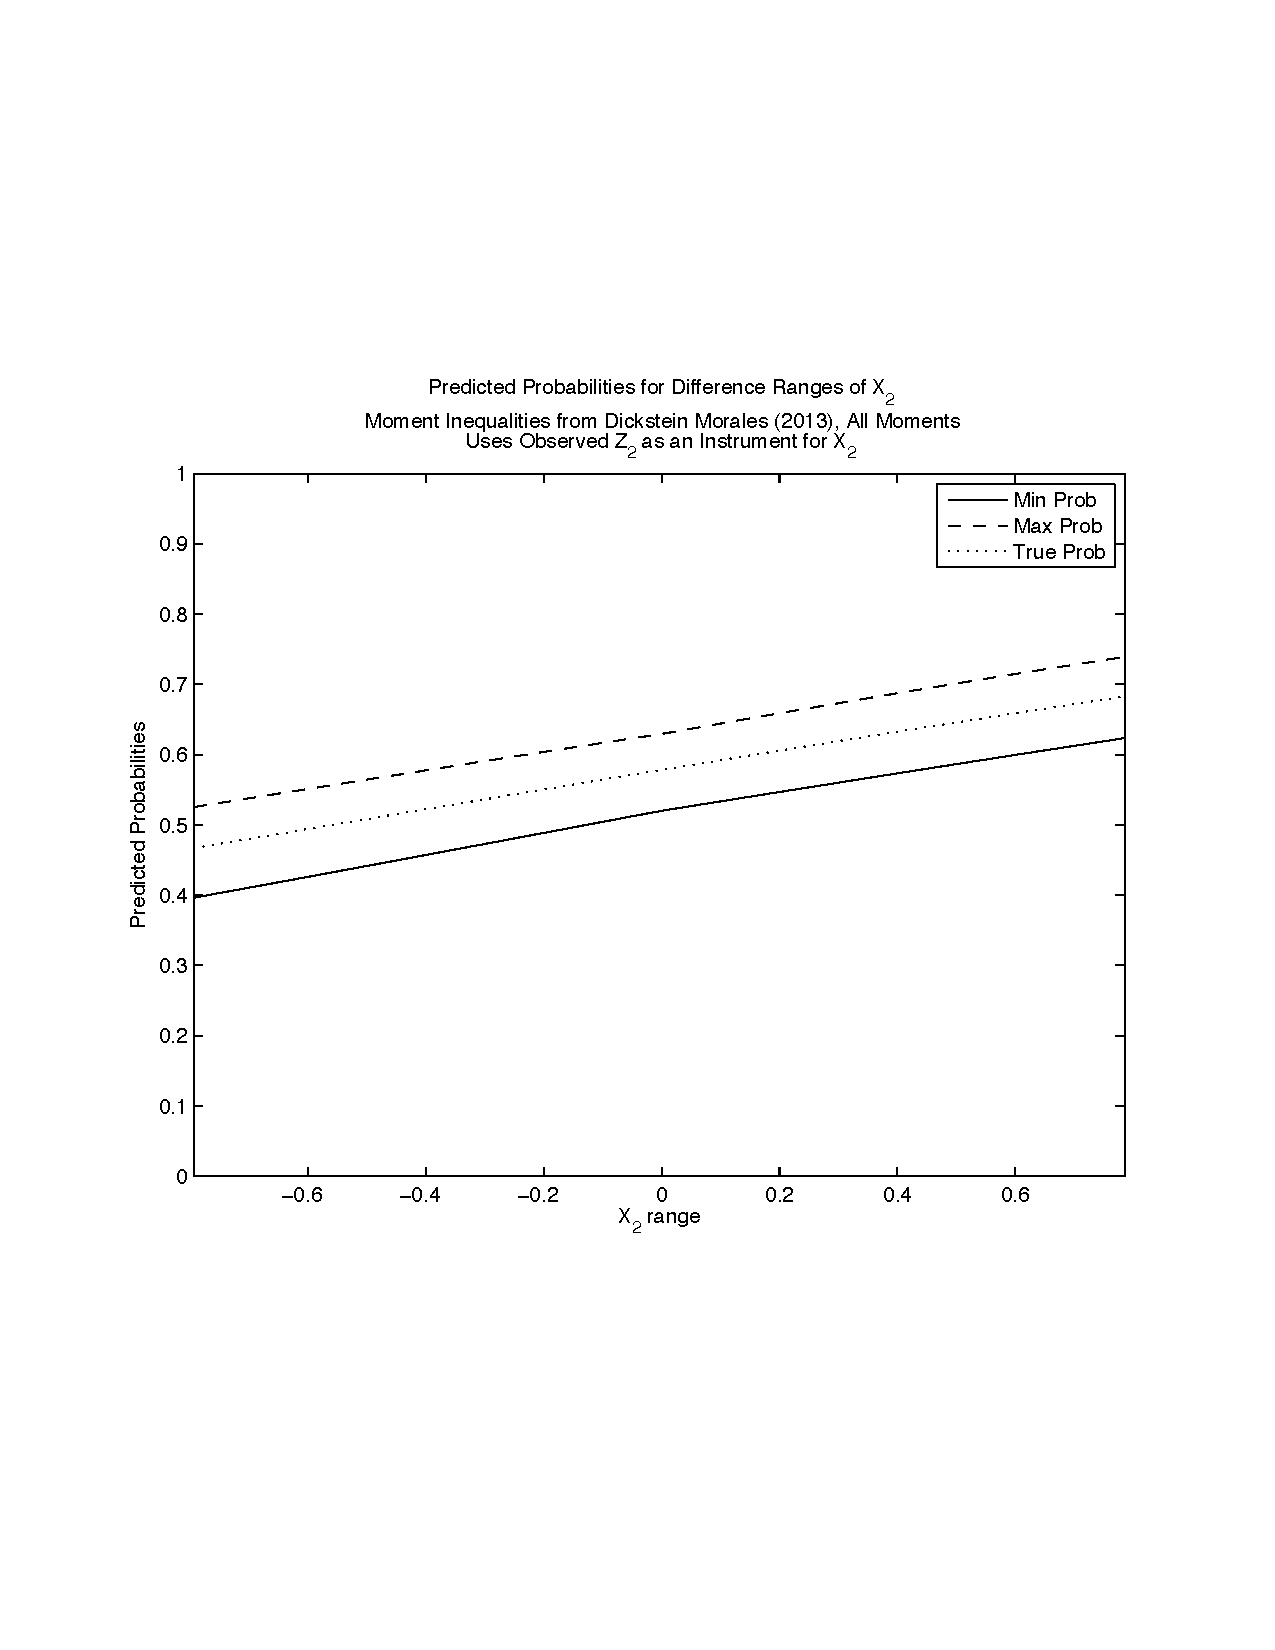
\includegraphics[width=.85\linewidth]{pred_prob_all.pdf}
\end{figure}

\end{frame}
%--------------------------------------------------------------------------------


%--------------------------------------------------------------------------------
\section{Misspecifictions}
%--------------------------------------------------------------------------------
\begin{frame}
\frametitle{Misspecifications of the Model: Endogenous Instrument}

\begin{itemize}
	\item Substitute Assumption 3 by Assumption 3(b):\\
	\bigskip
	\textbf{Assumption 3(b)} \textit{The distribution of $\Delta\varepsilon_{j}$ conditional on $(\Delta X_{j},\Delta \nu_{j})$ has support equal to $(-\infty,$ $\infty)$ and expectation equal to 0:
	\begin{align*}
	\mathbbm{E}[\Delta\varepsilon_{j}|\Delta X_{j},\Delta \nu_{j}]=0.
	\end{align*}}
	\item Then we can derive the following inequalities:
	\small
	\begin{align*}
	\mathbbm{M}^{q}_{s}(\beta)&=\mathbbm{E}\Bigg[\sum_{j\in\{0,1\}}\Bigg\{\Psi_{q}(\Delta X_{j})\Bigg(d_{j}\frac{F_{\nu}\big(-\beta\Delta X_{j}\big)}{1-F_{\nu}\big(-\beta\Delta X_{j}\big)}-d_{j'}\Bigg)\Bigg\}\Bigg]\geq 0,\\
	\mathbbm{M}^{q}_{r}(\beta)&=\mathbbm{E}\Bigg[\sum_{j\in\{0,1\}}\Bigg\{\Psi_{q}(\Delta X_{j})\Bigg(d_{j}\beta\Delta X_{j}+d_{j'}\mathbbm{E}\big[\Delta\nu_{j'}|\Delta\nu_{j'}\geq-\beta\Delta X_{j'}\big]\Bigg)\Bigg\}\Bigg]\geq 0,
	\end{align*}
	\normalsize
	\item If Assumption 3(b) does not hold, what are the properties of these inequalities?
\end{itemize}
\end{frame}

%--------------------------------------------------------------------------------
\begin{frame}
\frametitle{Misspecifications of the Model: Endogenous Instrument}

\begin{figure}[h!]
\centering 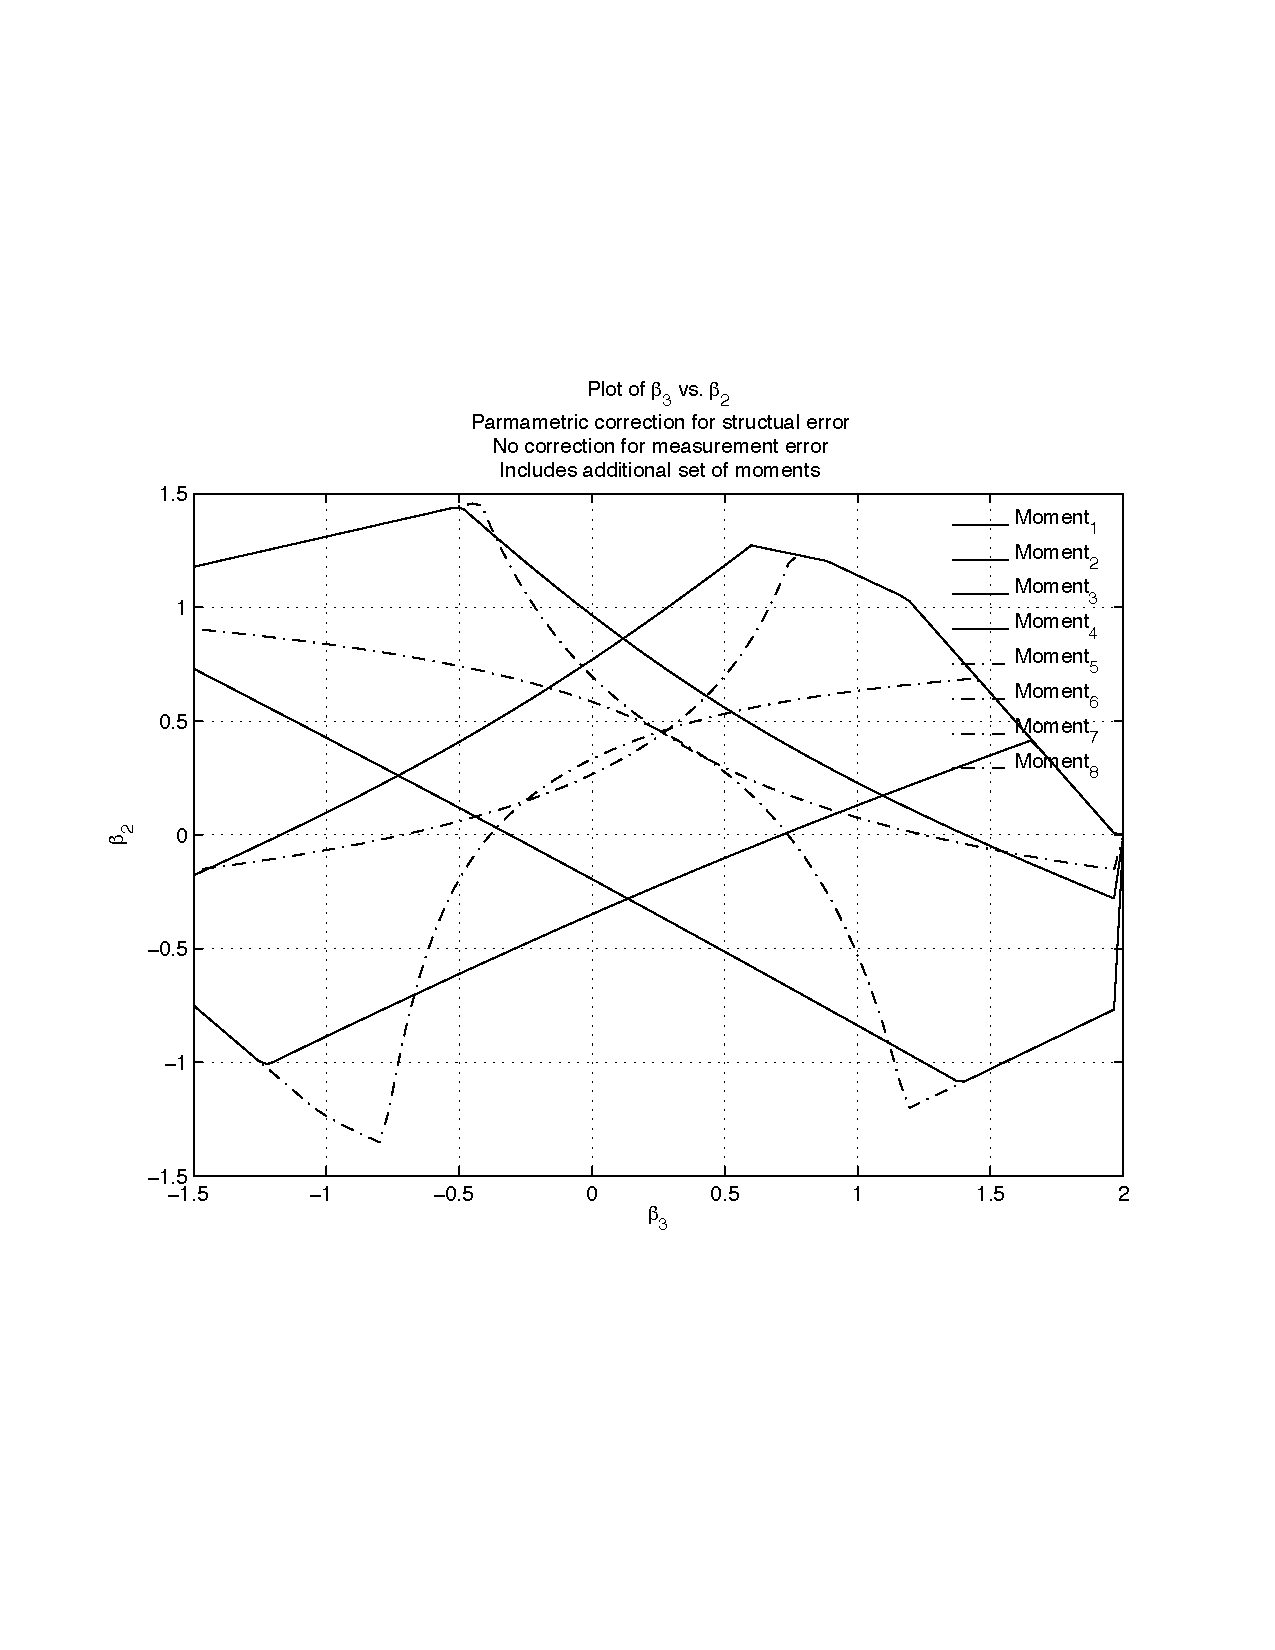
\includegraphics[width=.85\linewidth]{id_set_plots_endog_iv_all.pdf}
\end{figure}

\end{frame}
%--------------------------------------------------------------------------------
\begin{frame}
\frametitle{Misspecifications of the Model: Endogenous Instrument}

\begin{figure}[h!]
\centering 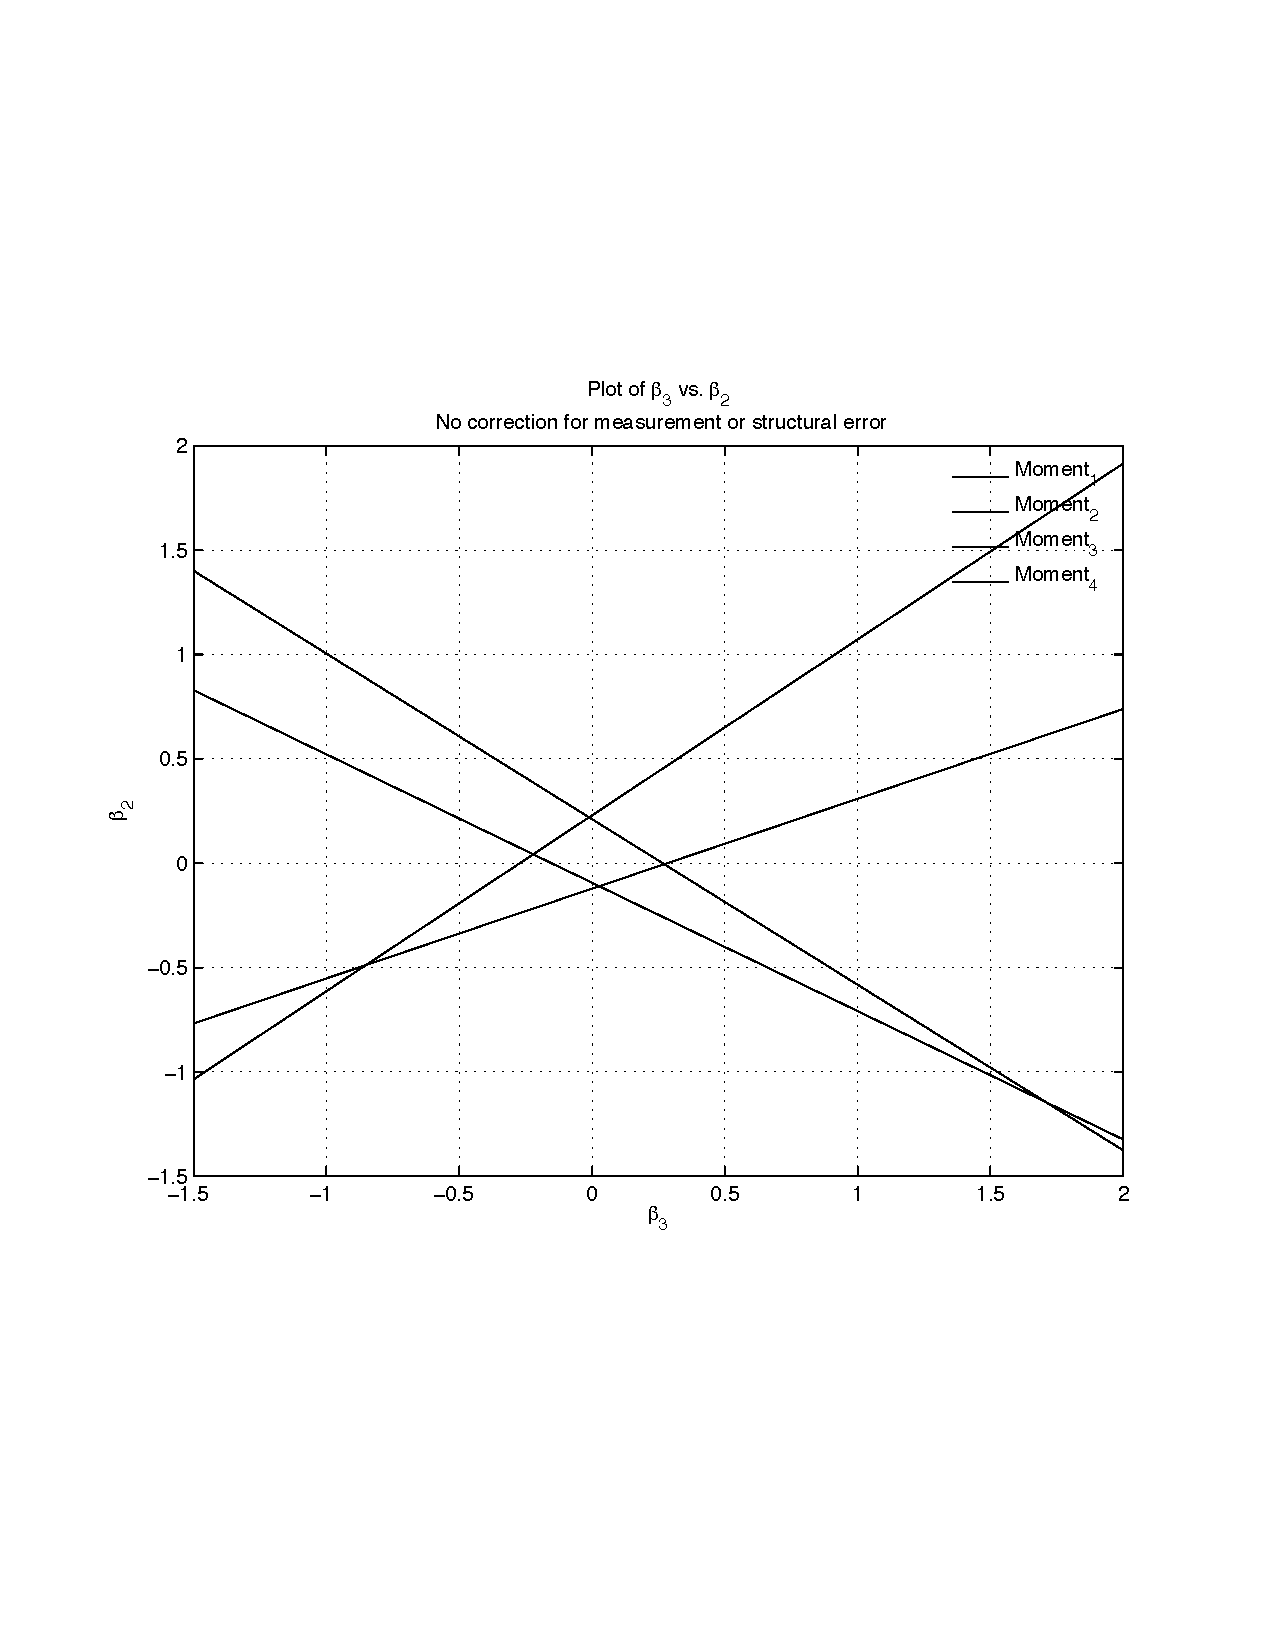
\includegraphics[width=.85\linewidth]{id_set_plots_endog_iv_pphi.pdf}
\end{figure}

\end{frame}
%--------------------------------------------------------------------------------
\begin{frame}
\frametitle{Misspecifications of the Model: No Structural Error}

\begin{itemize}
	\item Substitute Assumption 2 by Assumption 2(b):\\
	\bigskip
	\textbf{Assumption 2(b)} \textit{The marginal distribution function of $\Delta\nu_{j}$ has a degenerate distribution at $\Delta\nu_{j}$ = $0$.}
	\bigskip
	\item If Assumptions 1, 2(b), and 3 hold, then the score function moment inequality is irrelevant.
	\item The revealed preference inequality becomes
	\begin{align*}
	\mathfrak{M}^{q}_{r}(\beta)=\mathbbm{E}\bigg[\sum_{j\in\{0,1\}}\bigg\{\Psi_{q}(\Delta Z_{j})d_{j}(\beta_{1}\Delta Z_{1j}+\beta_{2}\Delta X_{j})\bigg\}\bigg]\geq 0,
	\end{align*}
\end{itemize}
\end{frame}

%--------------------------------------------------------------------------------
\begin{frame}
\frametitle{Misspecifications of the Model: No Structural Error}

\begin{itemize}
	\item Note that
	\small
	\begin{align*}
	\mathcal{M}^{q}_{r}(\beta)=\mathfrak{M}^{q}_{r}(\beta)+
	\end{align*}
	\begin{align*}
	\mathbbm{E}\Bigg[\sum_{j\in\{0,1\}}\Bigg\{\Psi_{q}d_{j'}\mathbbm{E}\big[\Delta\nu_{j'}|\Delta\nu_{j'}\geq-(\beta_{1}\Delta Z_{1j'}+\beta_{2}\Delta X_{j'})\big]\Bigg\}\Bigg].
	\end{align*}
	\normalsize
	\item If Assumption 2(b) does not hold, what are the properties of these inequalities?
\end{itemize}
\end{frame}
%--------------------------------------------------------------------------------
\begin{frame}
\frametitle{Misspecifications of the Model: No Structural Error}

\begin{figure}[h!]
\centering 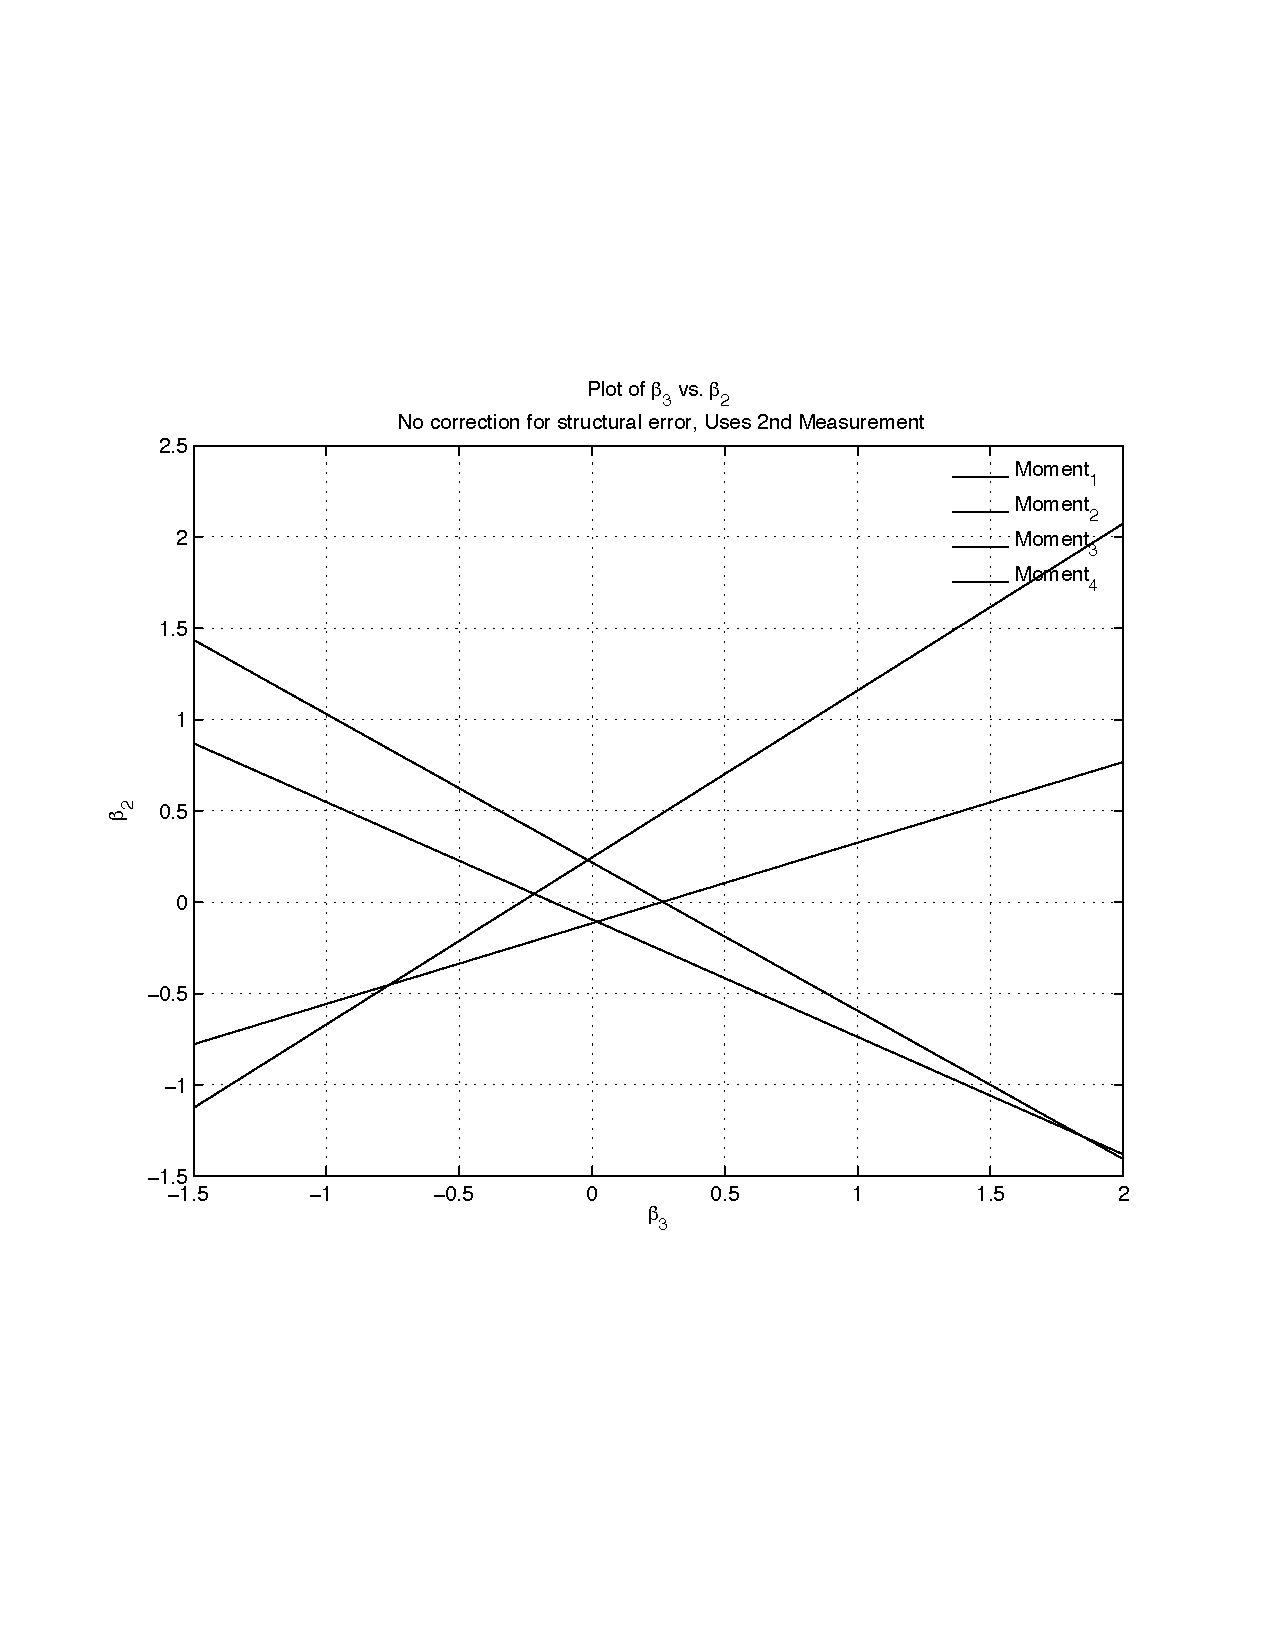
\includegraphics[width=.85\linewidth]{id_set_plots_pphi_ziv.pdf}
\end{figure}

\end{frame}
%--------------------------------------------------------------------------------

\begin{frame}
\frametitle{Misspecifications of the Model: No Structural Error}

\begin{figure}[h!]
\centering 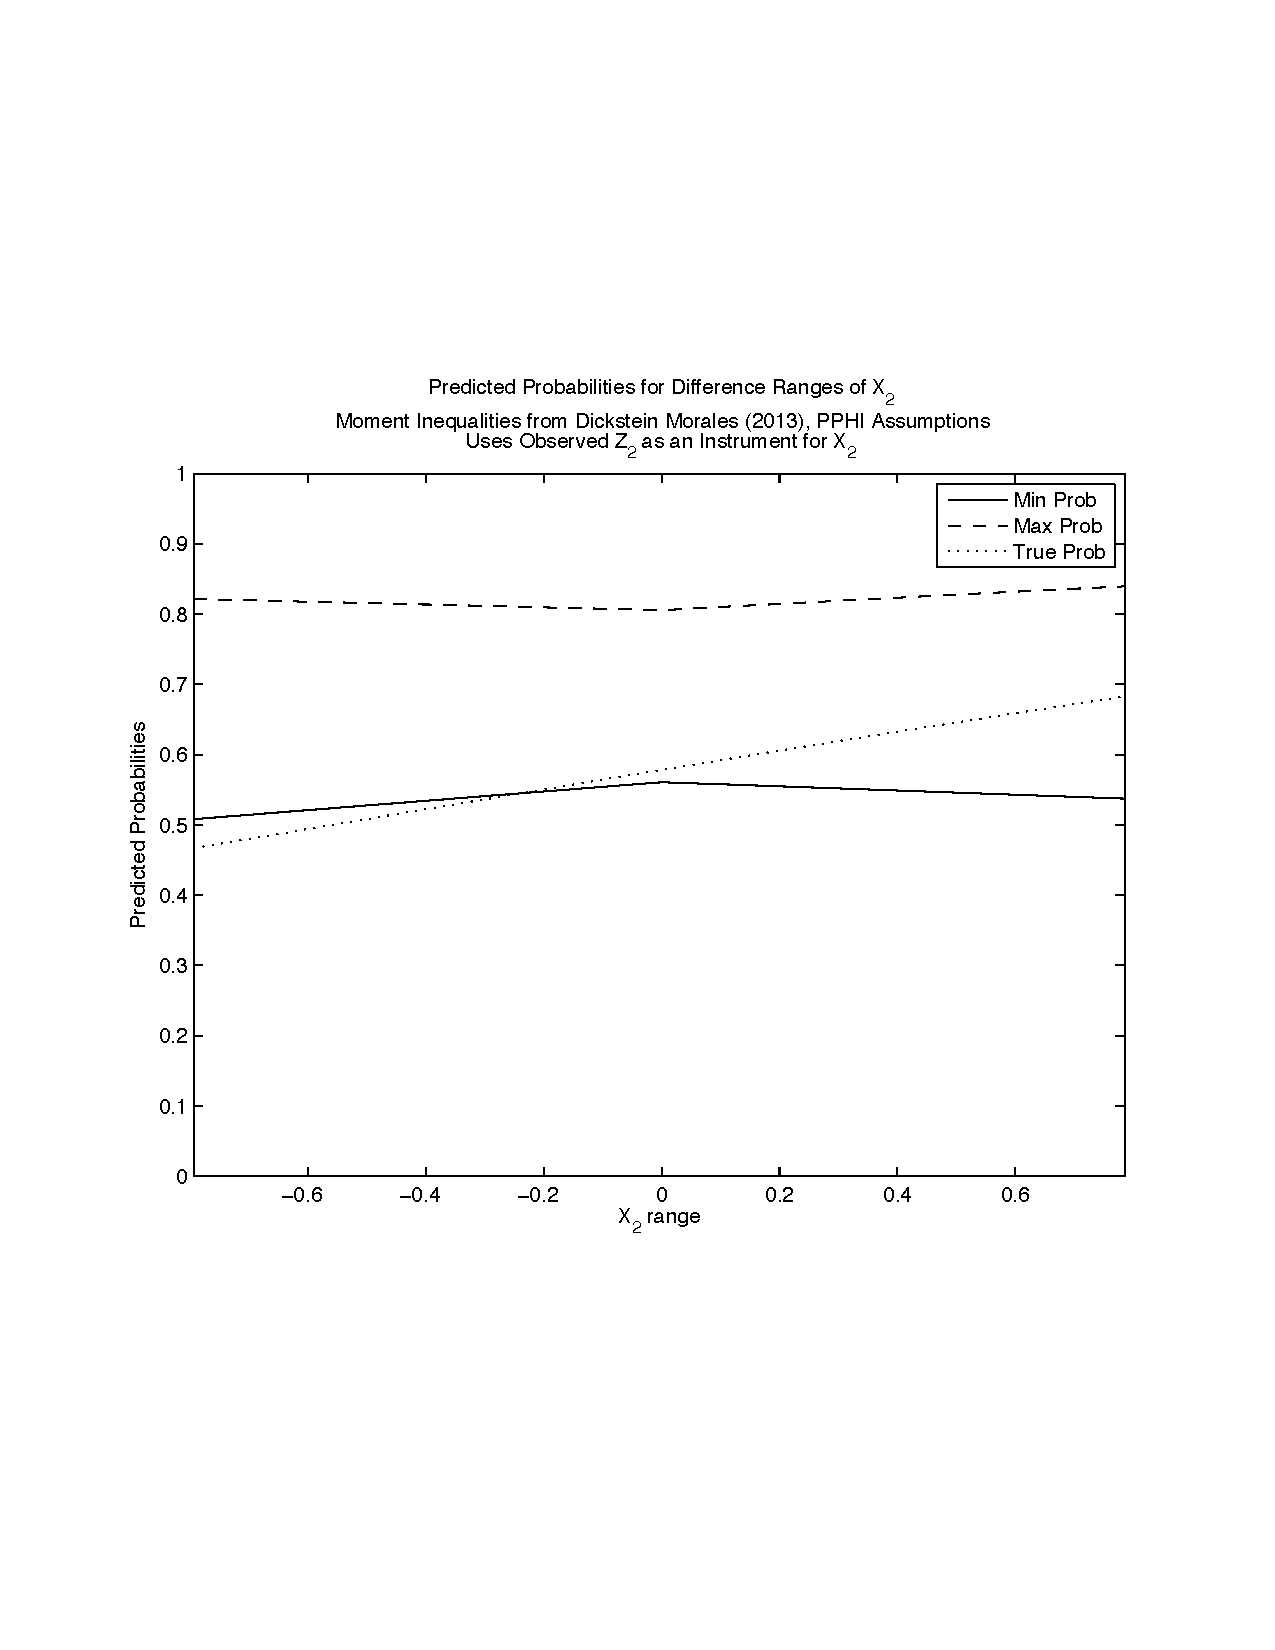
\includegraphics[width=.85\linewidth]{pred_prob_pphi.pdf}
\end{figure}

\end{frame}
%--------------------------------------------------------------------------------

\end{document}
